\section{Podaci o polenu}

\begin{frame}
    \frametitle{Podaci o polenu}

    \begin{columns}[c]
        % Leva kolona - slika
        \begin{column}{0.5\textwidth}
            \centering
            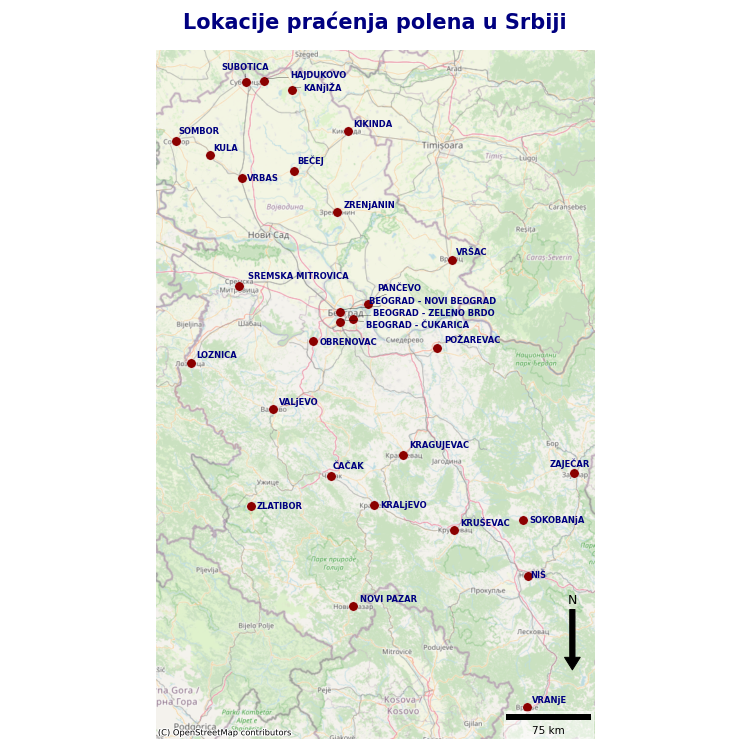
\includegraphics[width=\textwidth]{images/mapa_lokacija.png}
        \end{column}

        % Desna kolona - tekst
        \begin{column}{0.5\textwidth}
            \small
            Podaci su prikupljeni sa sajta 
            \href{https://data.gov.rs/sr/datasets/polen-objedinjeni-podatsi-od-2016-godine/}{\textbf{Portala otvorenih podataka Republike Srbije}}, 
            iz baze \textit{"Polen – objedinjeni podaci od 2016. godine"}.
            
            \vspace{0.3cm}

            Ova baza sadrži podatke o koncentraciji polena za 
            \textbf{29 mernih mesta} širom Srbije 
            i obuhvata \textbf{26 različitih alergena}.
        \end{column}
    \end{columns}

\end{frame}

\begin{frame}
    \frametitle{Primer merenja – Ambrozija (Požarevac)}

    \begin{center}
        % Prva slika
        \includegraphics[width=0.6\textwidth]{images/AMBROZIJA_POŽAREVAC_daily_concentration.png}

        % Druga slika
        \includegraphics[width=0.6\textwidth]{images/AMBROZIJA_POŽAREVAC_seasonal_concentration.png}
    \end{center}

\end{frame}


\begin{frame}
    \frametitle{Meteorološki parametri}

    \begin{columns}[c]
        % Leva kolona - slika
        \begin{column}{0.55\textwidth}
            \centering
            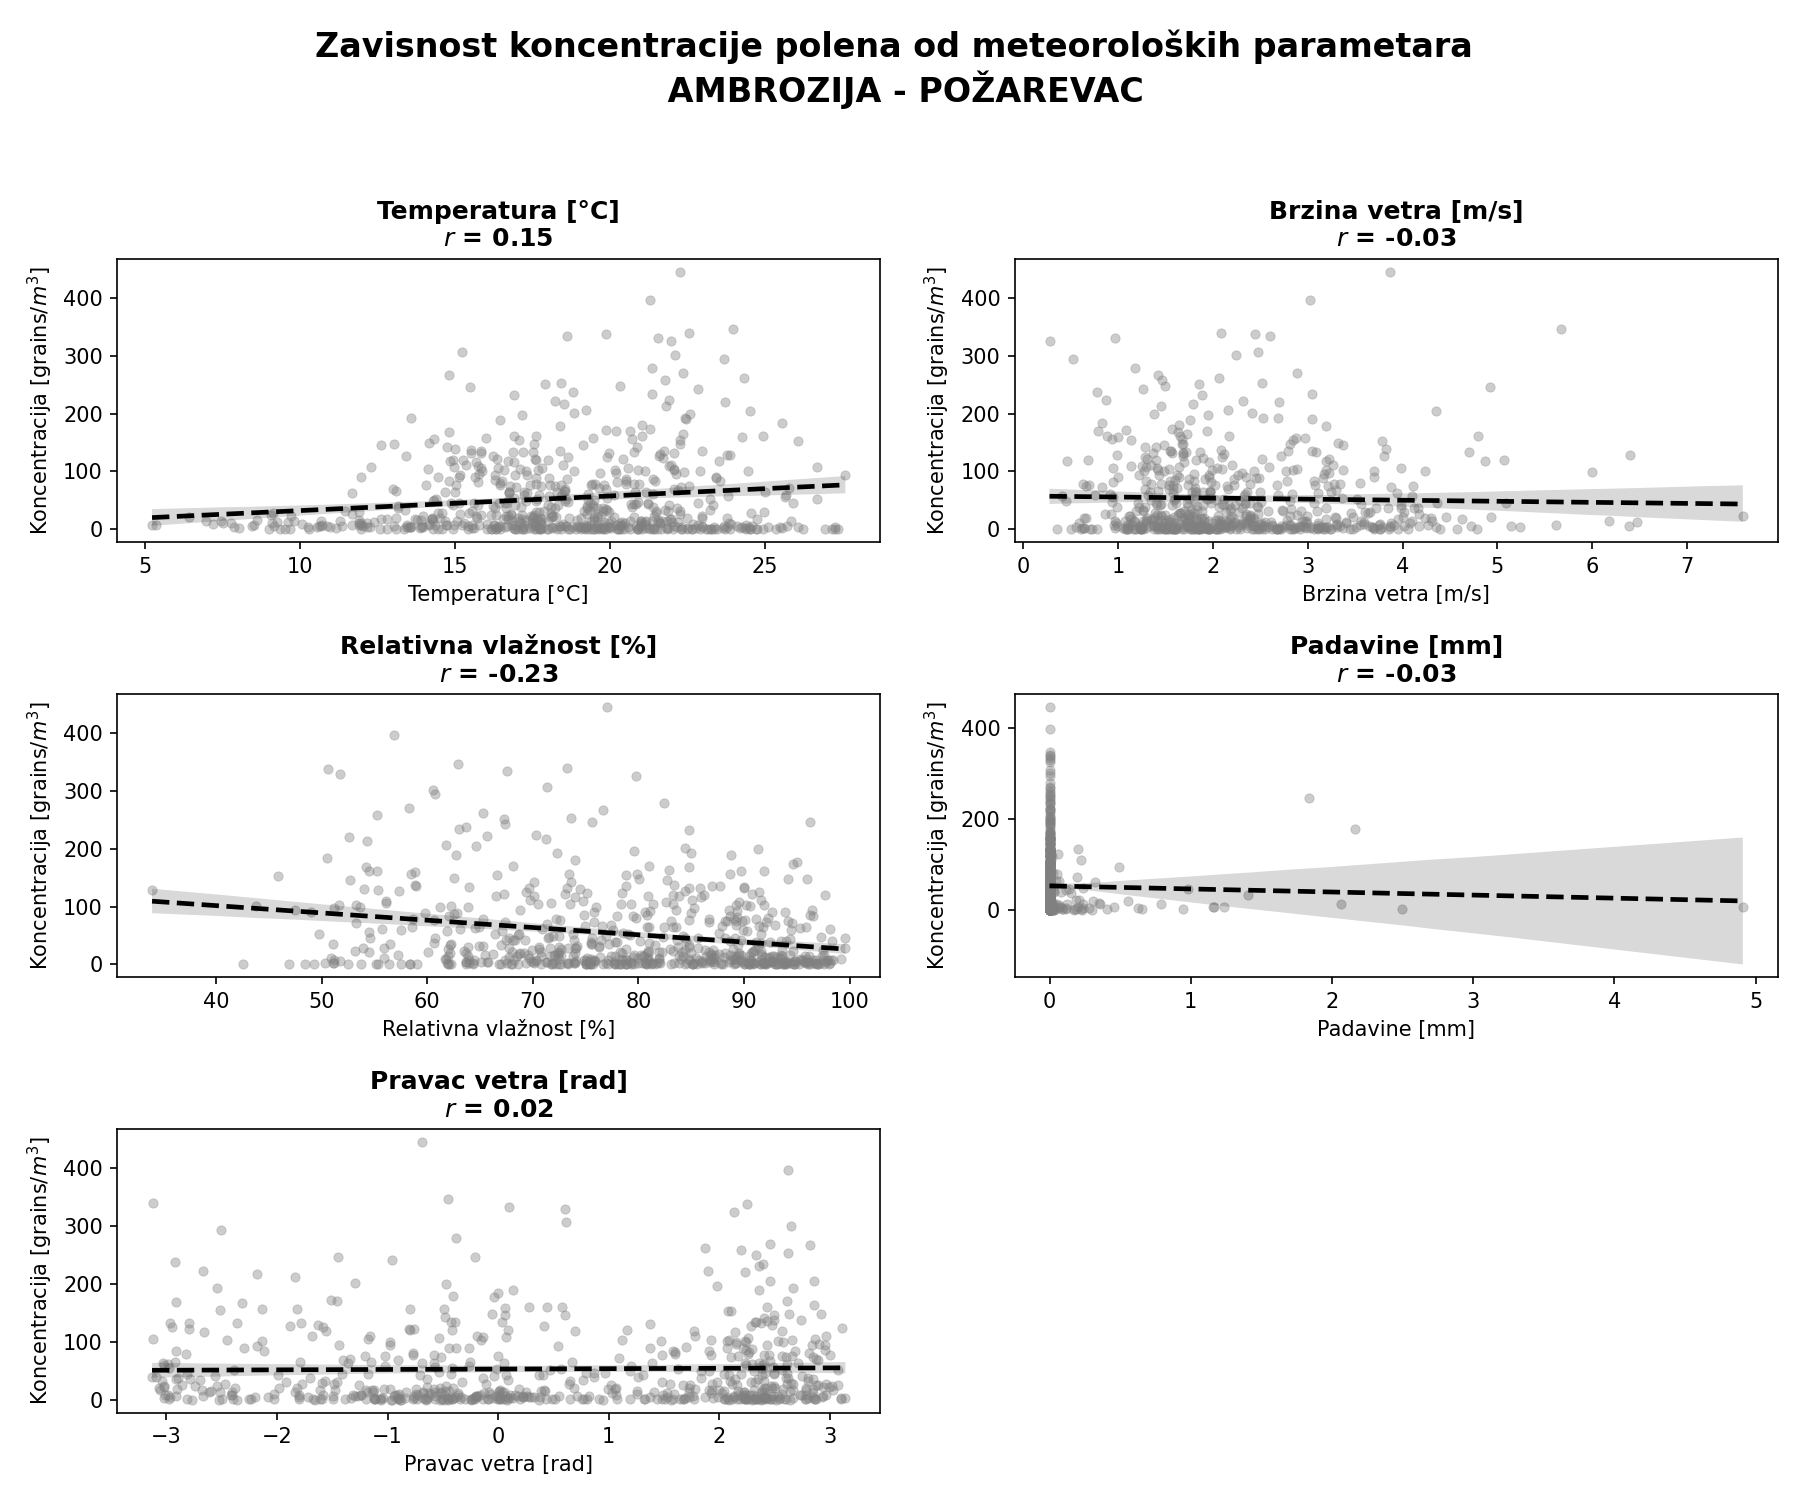
\includegraphics[width=\textwidth]{images/meteo.png}
        \end{column}

        % Desna kolona - tekst
        \begin{column}{0.43\textwidth}
            \small
            \textbf{Uz polenske podatke}, analizirani su i \textbf{meteorološki parametri} 
            koji značajno utiču na koncentraciju polena u vazduhu:
            \vspace{0.2cm}
            \begin{itemize}
                \item Temperatura vazduha \textbf{(+)}.
                \item Brzina vetra \textbf{(+)}.
                \item Vlažnost vazduha \textbf{(–)}.
                \item Padavine \textbf{(–)}.
                \item Pravac vetra.
            \end{itemize}
        \end{column}
    \end{columns}

\end{frame}





